\documentclass[output=paper]{LSP/langsci}  
\author{Lorenzo Spreafico\affiliation{Free University of Bozen-Bolzano}} 

\title{\mbox{\em s}-retraction in Italian-Tyrolean bilingual speakers: a preliminary investigation using the ultrasound tongue imaging technique}
% \title{\textit{s}-retraction in Italian-Tyrolean bilingual speakers: a preliminary investigation using the ultrasound tongue imaging technique}
\abstract{This paper presents a preliminary description of the articulation of /s/ in Italian as spoken by Italian-Tyrolean simultaneous and sequential bilingual speakers. The objective is to discuss whether they articulate /s/ differently. To this aim, articulatory differences across monolingual and bilingual speakers are commented upon, in particular focusing on s-retraction, which is attested to different degrees in Italian-Tyrolean simultaneous bilingual speakers and in Tyrolean-dominant sequential bilinguals, but not in Italian-dominant sequential bilingual speakers.
}

\maketitle 
\begin{document}
  
\section{Introduction}
South Tyrol - an Italian region located on the border with Austria and Switzerland - is characterized by societal bilingualism with two distinct linguistic communities - the Tyrolean and the Italian - that present asymmetries in their linguistic repertoires. The members of the Tyrolean community are multilingual and speak Tyrolean (\textsc{tyr}), an East Upper German dialect \citep{wiesinger_einteilung_1983,russ_central_1990}, as their first language, and standard German (\textsc{ger}; \citealt{ciccolone_lo_2010}) and regional Italian (\textsc{ita}; \citealt{mioni_litaliano_2001}) as their second and third language respectively. In contrast, the members of the Italian community are mostly monolingual and speak Italian: hardly anybody in the Italian community masters \textsc{tyr} and few members of the Italian community use \textsc{ger}, a language they learn at school. After years of segregation,\footnote{One relevant aspect of segregation of the two main linguistic communities is in the separated school system that operates within the province of South Tyrol. \citet[237]{woelk_educational_2008} note that the institution of the division along linguistic lines in the field of education is used by the political representatives of the Tyrolean community to protect “the German mother tongue against `foreign' influence and `mixture' with other languages”.} the degree of interaction between the Italian and the Tyrolean community is steadily increasing and the number of bilingual speakers is gradually growing.

In this research note, I focus on s-retraction, the phenomenon in which /s/ is realized as an 
%[ɕ]-like or as an [ʃ]-like sound. 
There is no previous research done on s-retraction in \textsc{ita} as spoken by mono- or bilingual speakers. Nevertheless quite often monolingual speakers of \textsc{ita} make fun of bilingual speakers from the Tyrolean community because they articulate a backed sound instead of the Italian alveolar [s]. For example, they are said to utter 
%['ɕkwillo] and ['ʃkonto] 
instead of standard Italian ['skwillo] `ring' and ['skonto] `sale'. s-retraction in \textsc{ita} as spoken by bilingual speakers might be due to an influence from the Tyrolean substratum, since in this dialect the voiceless sibilant is articulated with the body of the tongue raised against the hard palate whenever it is followed by a consonant. This is attested in word initial position, as well as in medial and final position \citep{alber_regional_2001,alber_silbenonset_2005}. Consequently, s-retraction might be indexically important to discriminate between monolingual and bilingual speakers of \textsc{ita} from South Tyrol.

\section{Informants and data collection}
To investigate preliminarily the question of the possible sociophonetic relevance of /s/-retraction in \textsc{ita}, I selected four speakers aged between 22 and 27 all born and living in Meran. In order to exclude possible gender-induced variation (\cite{fuchs_differences_2011}), I only selected female speakers. All informants had comparable socio-demographic status but different rates of bilingualism as inferable on the basis of two parameters: the age of first exposure to \textsc{ita} and/or \textsc{try}; and the rate of dual language exposure. According to these parameters the sample included two late sequential (LS) bilingual speakers and two simultaneous bilingual (SB) speakers. The late sequential speaker LS1 is an almost monolingual speaker of \textsc{ita} who stems from a strictly monolingual Italian family and attended only the Italian section of the South Tyrolean school system. The late sequential speaker LS2 is a Tyrolean-dominant informant who grew up in a Tyrolean-speaking family and attended the German school section only. The simultaneous bilingual speakers SB1 and SB2 originate from two different bilingual families, have both been exposed to \textsc{ita} and \textsc{try} since their birth, and attended the Italian as well as the German section of the South Tyrolean school system.

In order to describe /s/-retraction, I employed the Ultrasound Tongue Imaging (UTI) technique \citep{stone_guide_2005}. UTI involves the use of an ultrasound transducer fixed under the speaker’s chin to obtain images of the tongue. The system I used is based on the SonixTablet machine equipped with a microconvex probe recording up to 160 fps at a variable depth of 8 mm to 9 mm (according to the anatomy of the speaker). The machine was synchronized to the audio via the Ultrasonix module in the AAA software by Articulate Instruments. All speakers were recorded in the Alpine Laboratory of Phonetics and Phonology (ALPs) at the University of Bozen. Shortly before the experiment, all informants received detailed instructions on the test procedure. In order to activate the bilingual mode \citep{grosjean_transfer_1998}, instructions were given both in Italian and in Tyrolean. Each speaker was instructed to read aloud a list of sentences prompted on a screen. The prompt list consisted of 40 Italian items with word initial and word internal /s/, /sV/, /sC/ (C=\{p, t, k\}; V=\{a, i, u\}) groups. The prompt list also contained distractors and three Tyrolean words “schtruuze” `(kind of) bread', “odminischtrativor” `administrative', “schtrimpf” `stockings'. For each informant, I was able to obtain a minimum of one to a maximum of three repetitions of the whole sentence list, depending on their resistance to the probe stabilization helmet I used.

\section{Data analysis}
For the within-speaker comparison, I followed the proposal in \citet{davidson_comparing_2006}: firstly, I calculated the smoothing spline estimates; secondly, I computed the Bayesian confidence intervals for each set of curves. My aim was to contrast the tongue shape of Italian /s/ in /sV/ sequences vs. the tongue shape of Italian /s/ in /sCV/ sequences to test if, as documented for Tyrolean, the consonant following the sibilant triggered /s/-retraction in the productions of simultaneous bilinguals and/or of the Tyrolean-dominant sequential bilingual.

\figref{fig:1} shows the results of the comparison of /s/ in the two words /'sano/ `sane' and /'skanno/ `I slaughter' for the Italian-dominant speaker. For the purpose of this paper, the main regions of interest are the rightmost part of the tongue, corresponding to the anterior part of the tongue including the blade and tip, and the central part of the tongue, corresponding to the body. The tracings display a tip-down post-alveolar constriction, with the apex of the tongue stopping before the point of contact for /t/ as well as some instances of tongue flexion in the pre-palatal region. The constriction location for /s/ is kept constant across repetitions, but the tongue body is kept higher in /'skanno/ and pointing to the constriction location for the following velar stop. The interaction effect graph confirms the visual impression and indicates that for both stimuli, the tongue blade and tip have comparable contours while the tongue body significantly differs.

\begin{figure}  
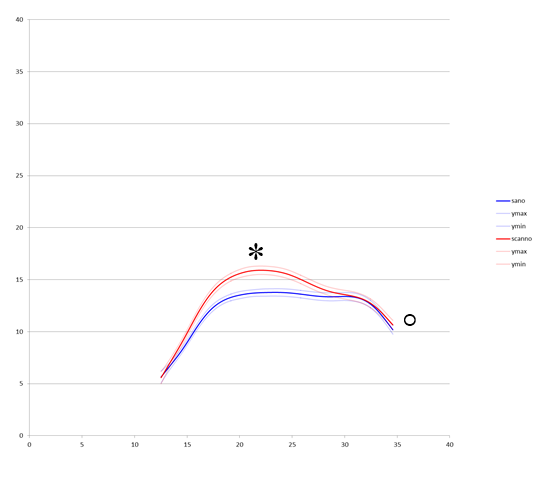
\includegraphics[width=0.4\textwidth]{illustrations/sprea_fig1a}~
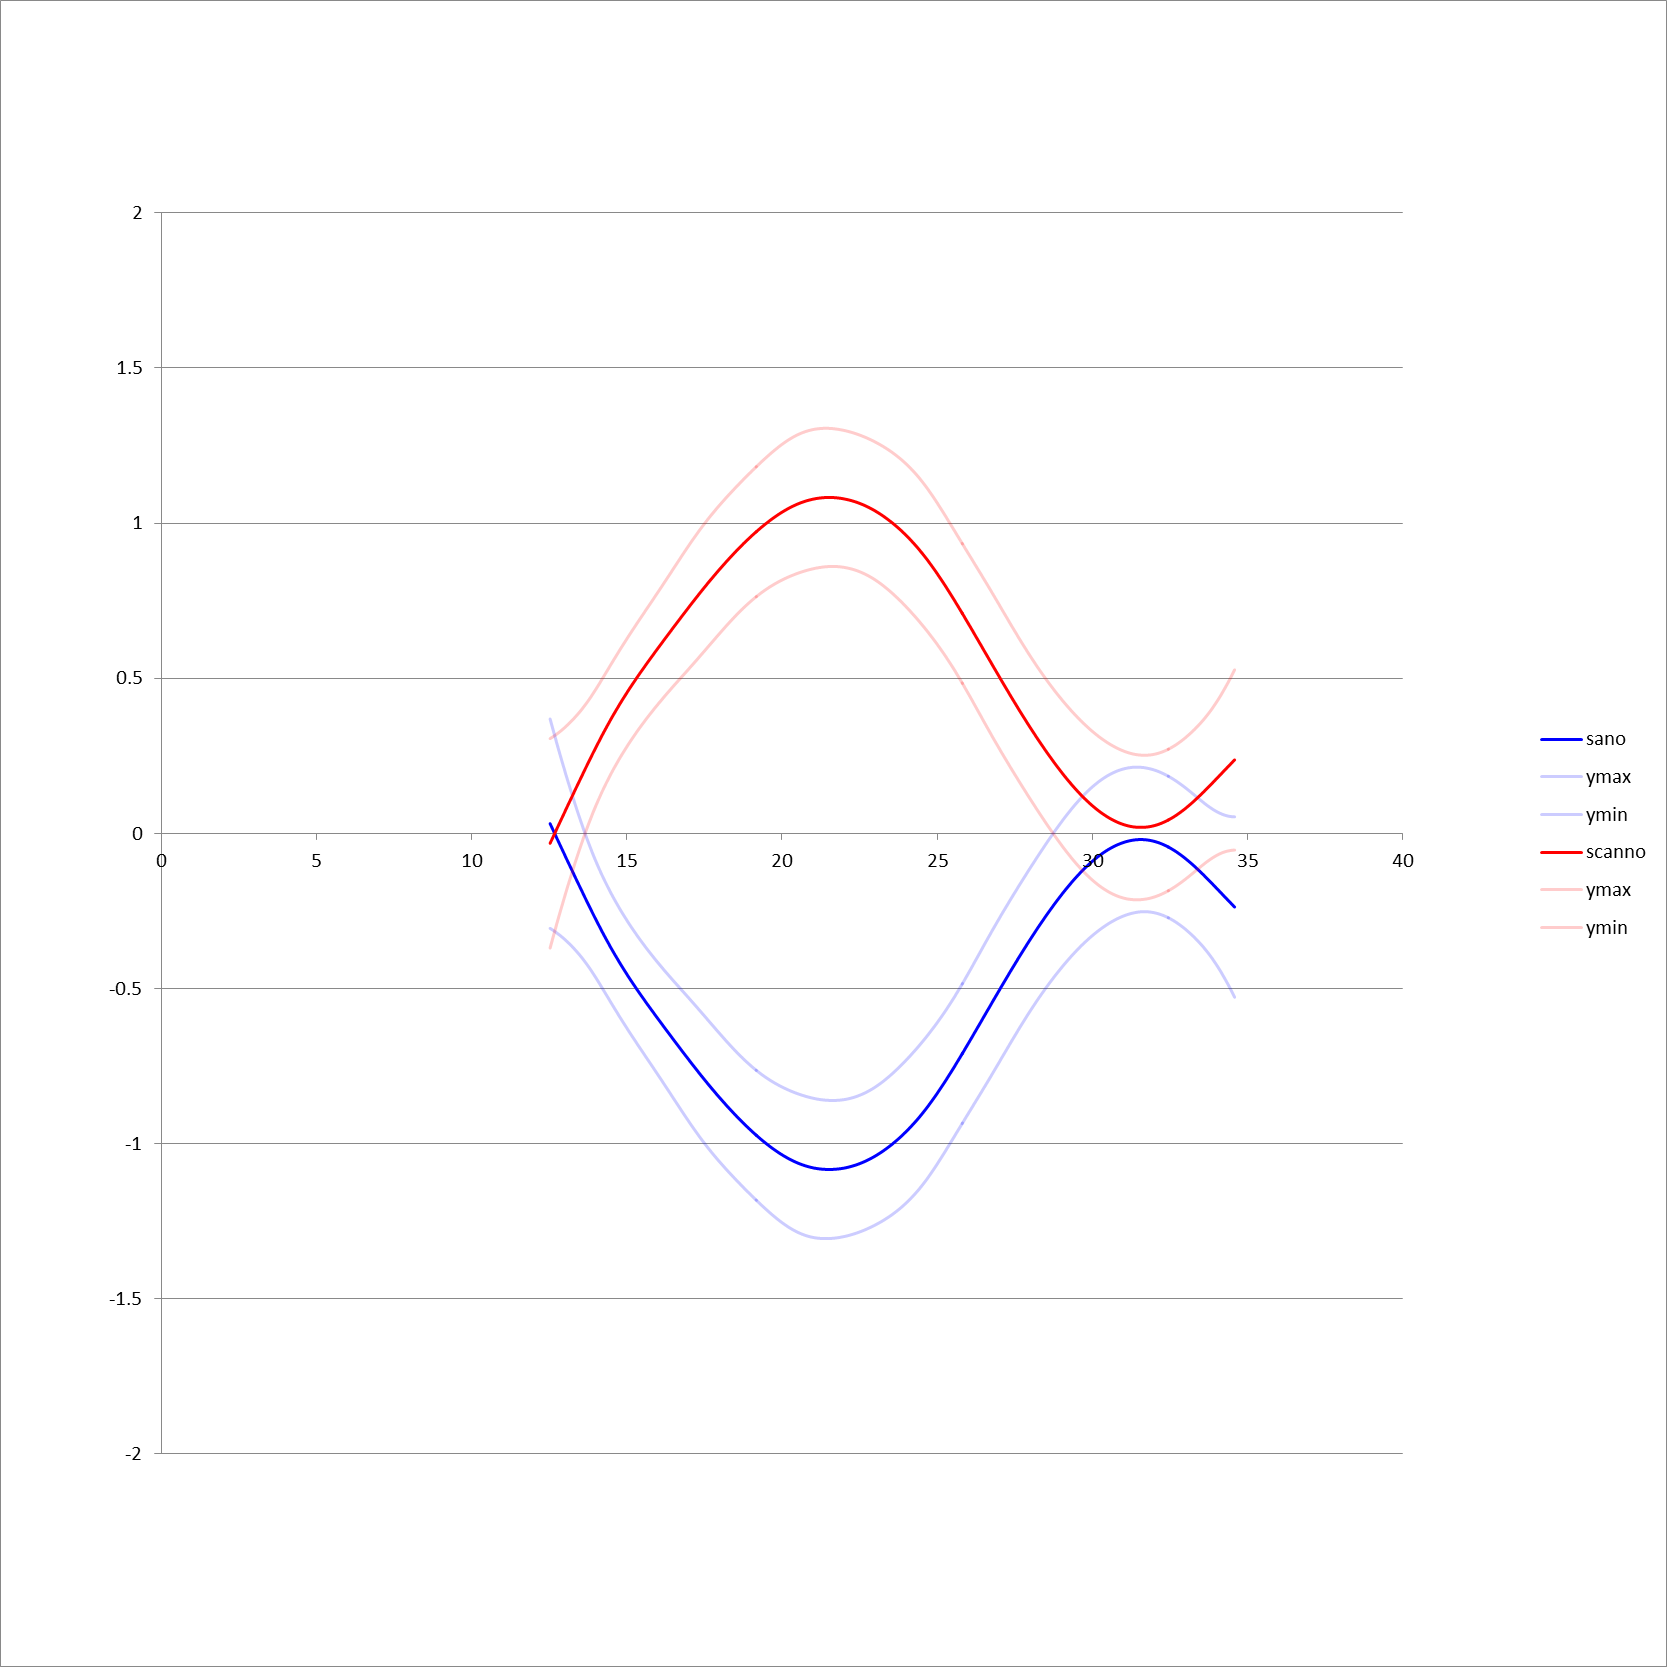
\includegraphics[width=0.4\textwidth]{illustrations/sprea_fig1b}
\label{fig:1}   
\caption{Smoothing spline estimate with 95\% Bayesian confidence interval (left) and interaction effects (right) for comparison of the mean curves for /s/ in /'sano/ (blue) and /'skanno/ (red) for subject LS1. No palate shapes were exported for this study, but in each Figure * and ° point to the place of articulation for /t/ and /k/ respectively. Tip and blade are to right; root is to left. In the Bayesian confidence interval graph, when confidence intervals of the main effects curves overlap, the differences between the two curves are not significant.}
\end{figure}

\begin{figure}
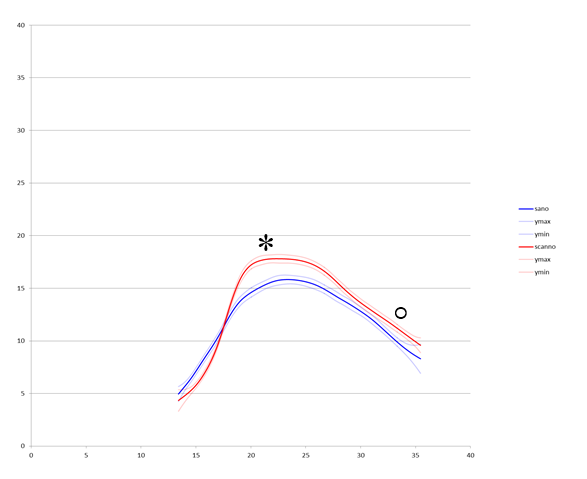
\includegraphics[width=0.4\textwidth]{illustrations/sprea_fig2a}~
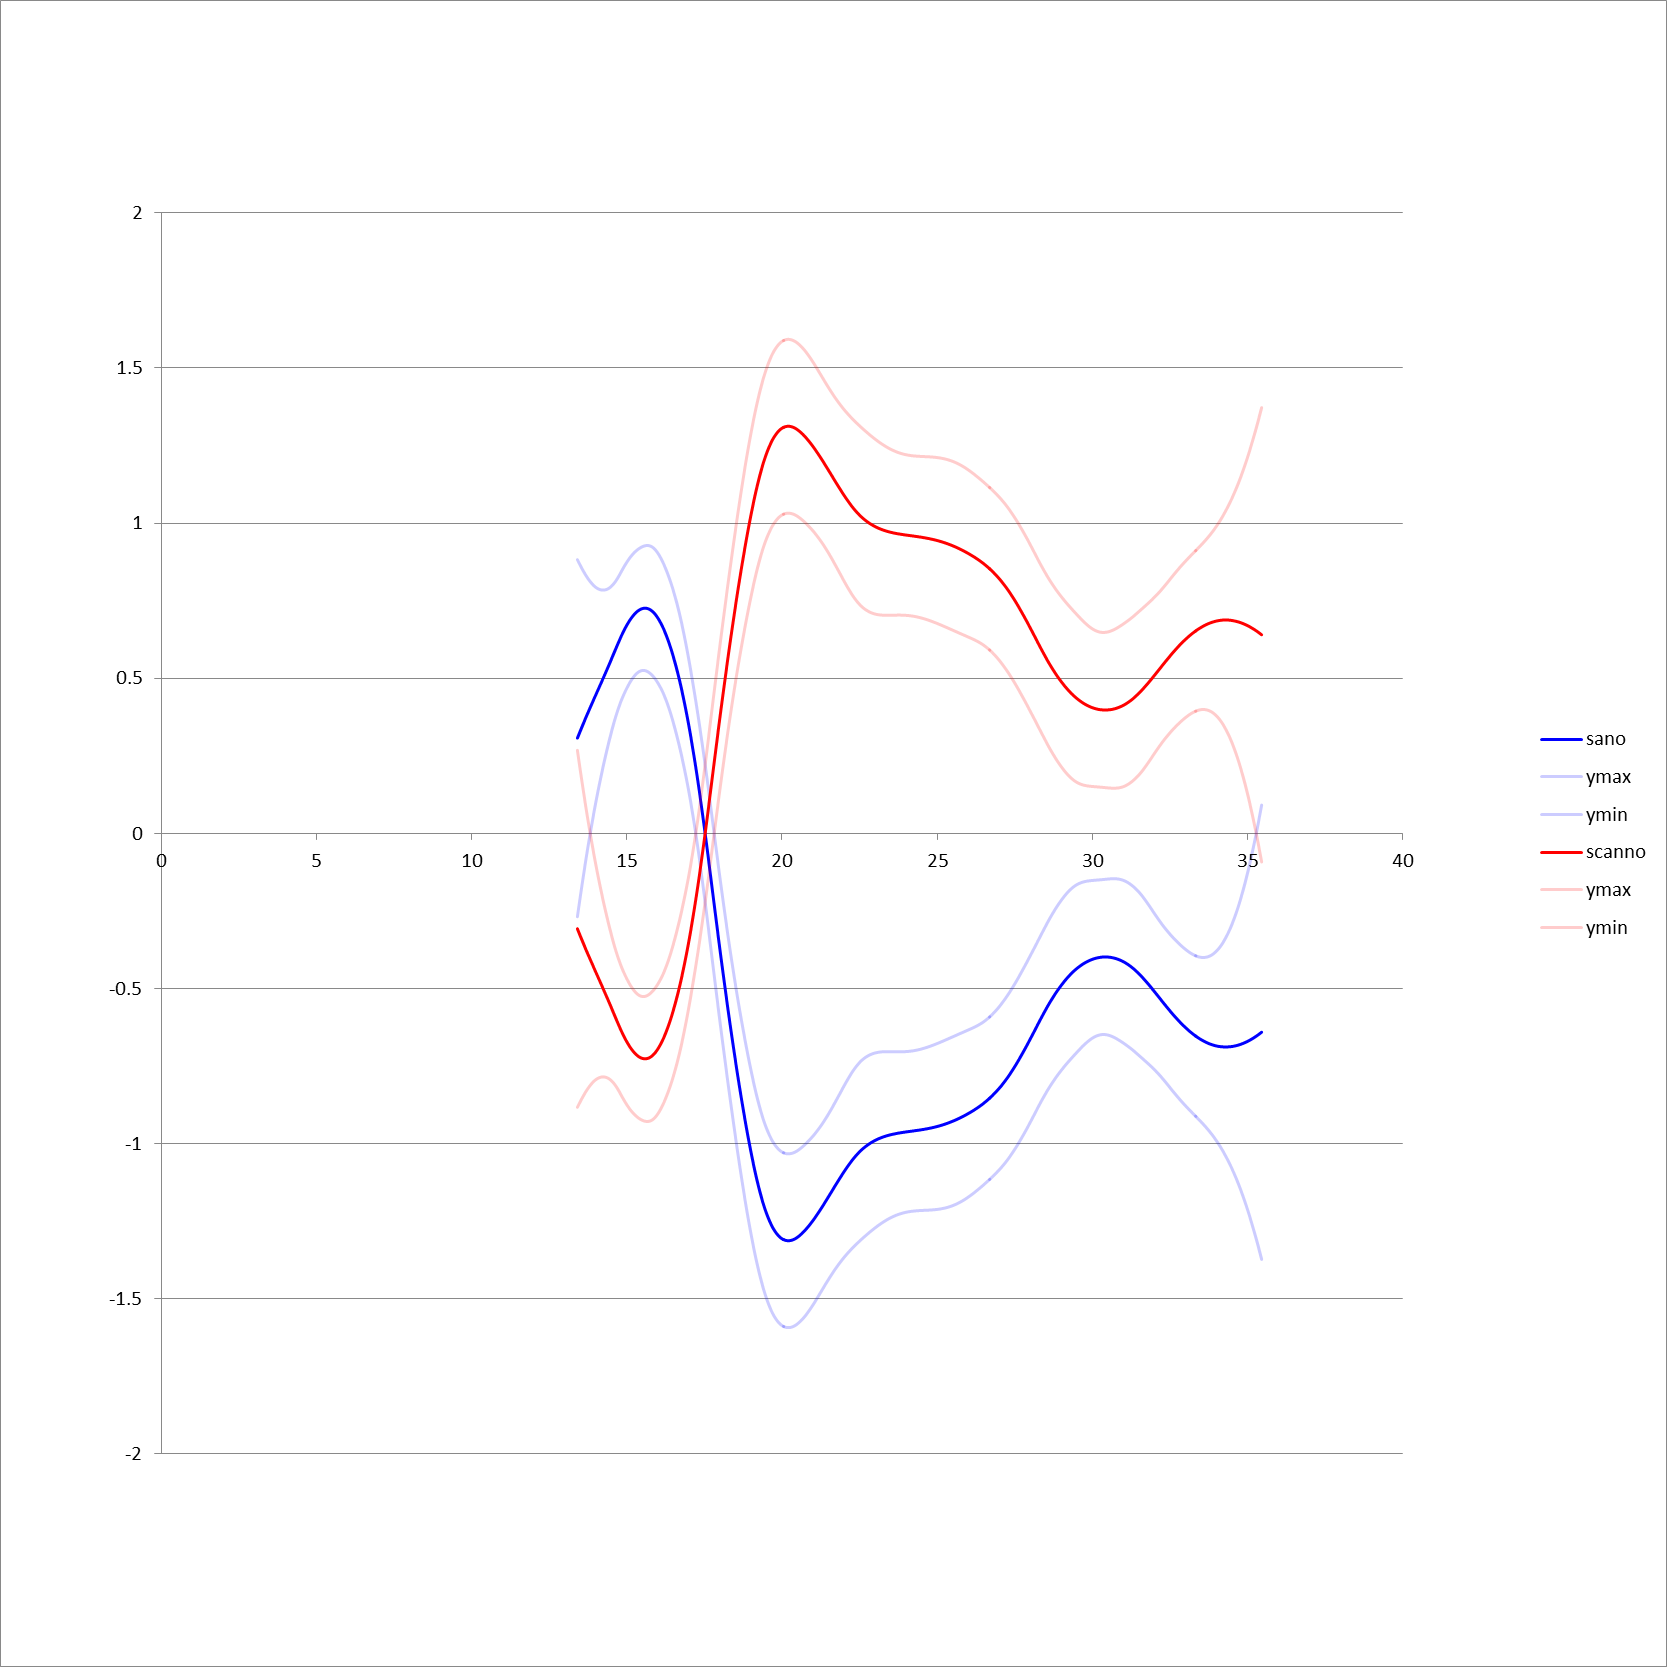
\includegraphics[width=0.4\textwidth]{illustrations/sprea_fig2b}
\label{fig:2}   
\caption{Smoothing spline estimate and interaction effects for subject LS2.}
\end{figure}


\figref{fig:2} displays data for the Tyrolean-dominant speaker. Visual inspection, confidence intervals and the interaction effect graph show that the silhouettes are significantly different for the entire length of the tongue. With regard to the /s/ in /'sano/, the posterodorsum is raised towards the hard palate and the anterodorsum and the tip are down. Regarding the /s/ in /'skanno/, the tongue body, blade and tip are higher, while the root is lower. There is an increased constriction degree in the velar region.

\figref{fig:3} shows data for the simultaneous bilingual speaker SB1. Notwithstanding the visual impression of affinity and notwithstanding the tongue tip pointing to the same constriction location in the alveolar area for both smoothed profiles, tracings are significantly different as displayed by the interaction effect graph. Regarding the tongue shape of /s/ in /'skanno/, the blade and tip are somehow lower than in /'sano/, while the body is higher and pointing to the hard palate. In /'sano/, the tongue body is lowered in the pre-palatal region thus showing tongue flexion.

  
\begin{figure}
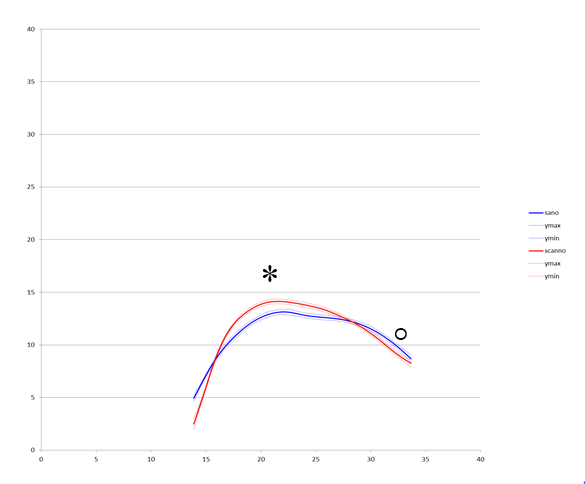
\includegraphics[width=0.4\textwidth]{illustrations/sprea_fig3a}~
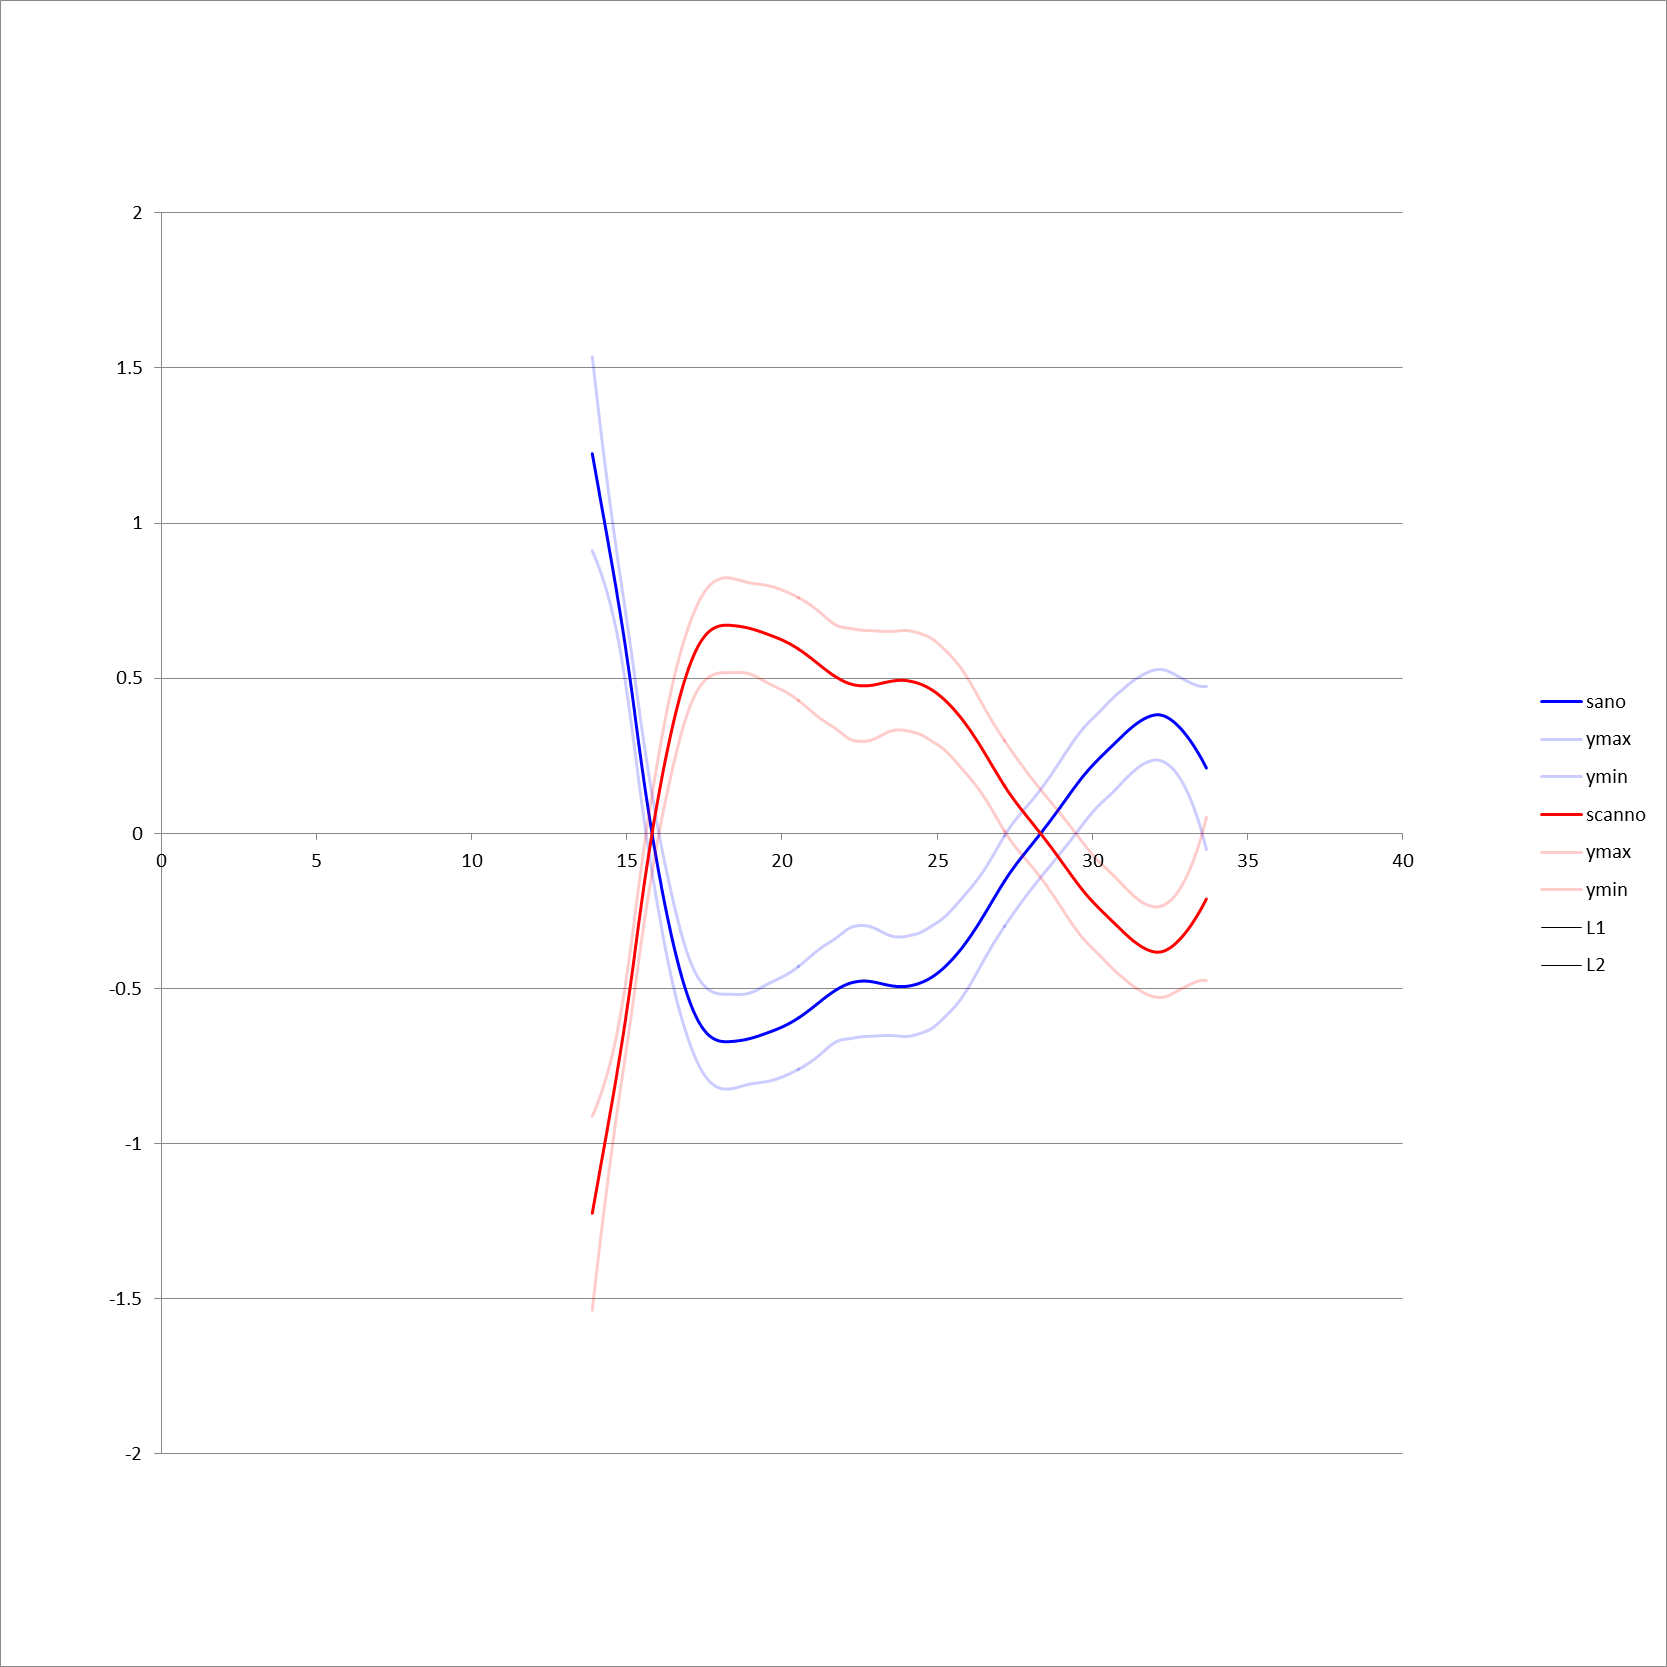
\includegraphics[width=0.4\textwidth]{illustrations/sprea_fig3b}
\label{fig:3}   
\caption{Smoothing spline estimate and interaction effects for subject SB1.}
\end{figure}

\figref{fig:4} presents data for the simultaneous bilingual speakers SB2. Visual investigation of the smoothing spline estimate shows almost coincidence of tongue profiles. The confidence intervals and the interaction curves confirm that there is no significant difference anywhere in the profiles, except for a few points at the tongue blade and tip and, to a lesser extent, two points in the postero-dorsum. The /s/ of /'skanno/ is articulated keeping the tongue apex slightly higher than in /'sano/.

  
\begin{figure}
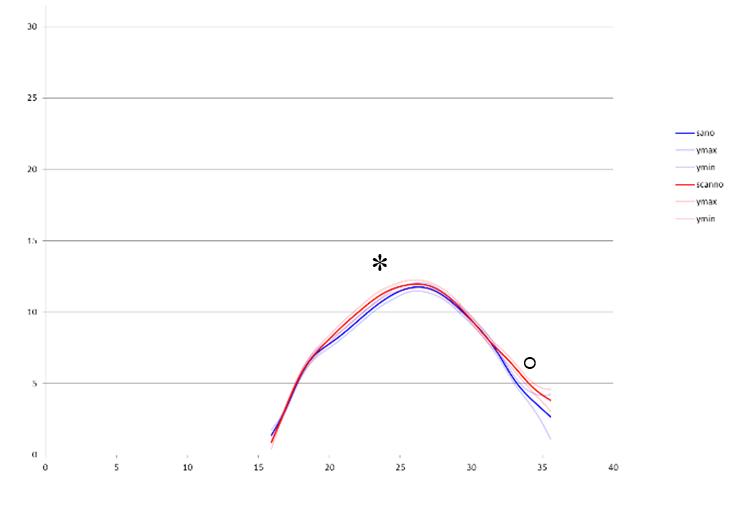
\includegraphics[width=0.4\textwidth]{illustrations/sprea_fig4a}~
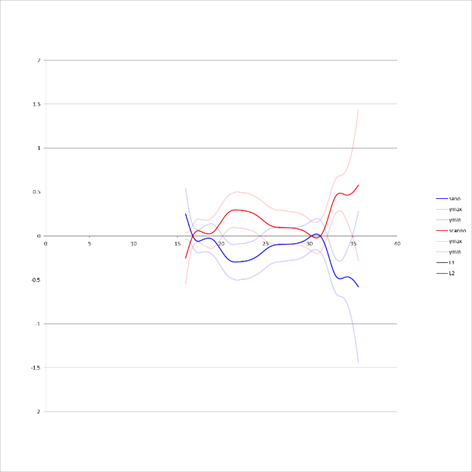
\includegraphics[width=0.4\textwidth]{illustrations/sprea_fig4b}
\label{fig:4}   
\caption{Smoothing spline estimate and interaction effects for subject SB2.}
\end{figure}

\section{Data discussion}
Figures 1-4 demonstrate that as far as Italian /s/ in /sV/ vs. /sCV/ sequences are concerned, the Italian-dominant sequential bilingual speaker LS1 does not differentiate the location nor the degree of constriction for the tongue tip and blade. Conversely, the Tyrolean-dominant speaker and the simultaneous bilingual speakers all display differentiated tongue apex profiles for /s/. Such dissimilarities are reflected in the interaction effects, whose absolute difference values are higher in the Tyrolean-dominant informant than in the simultaneous bilinguals.

Besides, and again with respect to tongue apex differences, it impressionistically emerges that the Italian-dominant sequential bilingual speaker presents apical articulation, which contrasts with laminal articulation in the Tyrolean-speaking informants.

Figures 1-4 also display that all speakers differentiate the tongue body position and keep it higher for /s/ in /'skanno/ than for /s/ in /'sano/. This evidences coarticulatory sensibility of /s/ to the subsequent velar stop. However, the values of interaction effects are more relevant for the late sequential bilinguals than for the simultaneous bilinguals. While this is not surprising for LS1 (as apical fricatives are less resistant to coarticulation than laminals; \citealt{hardcastle_lingual_1999}), this is of interest for LS2 as this might indeed reveal an influence from the Tyrolean substratum.

In order to test if this is the case and to investigate the possible retraction for the Italian sibilant, I contrasted the tongue shapes for /s/ in Italian and Tyrolean in a comparable phonetic environment. Unfortunately in the dataset there were no Tyrolean words containing the cluster /sk/ that I could have contrasted with the word /'skanno/ I commented on in the previous figures, so I used tracings of the fricative taken from Italian “castra” `s/he castrates' and from Tyrolean “odminischtrativor” `administrative'.

\begin{figure}
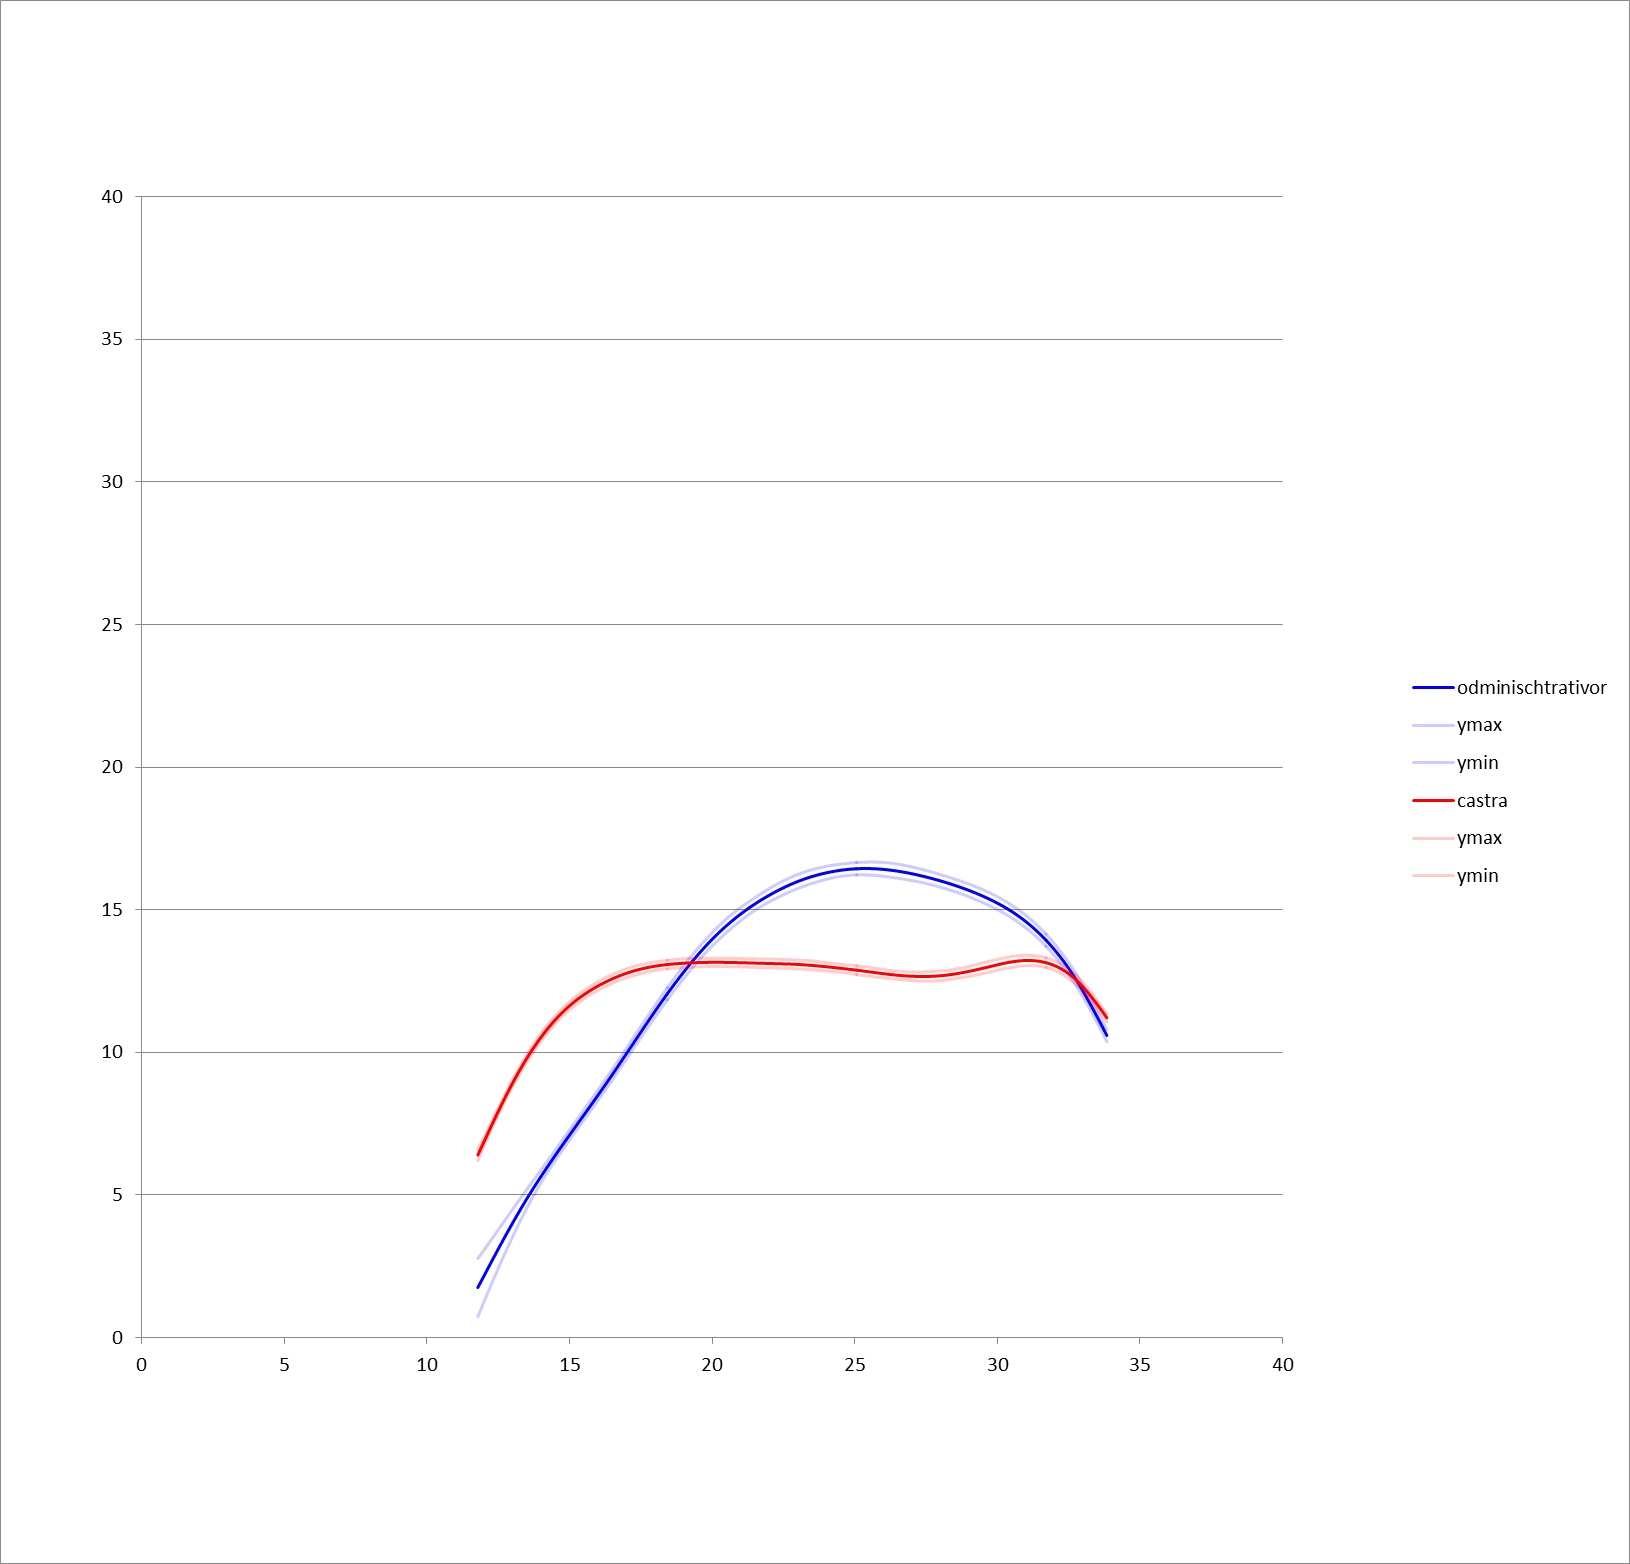
\includegraphics[width=0.4\textwidth]{illustrations/sprea_fig5a}~
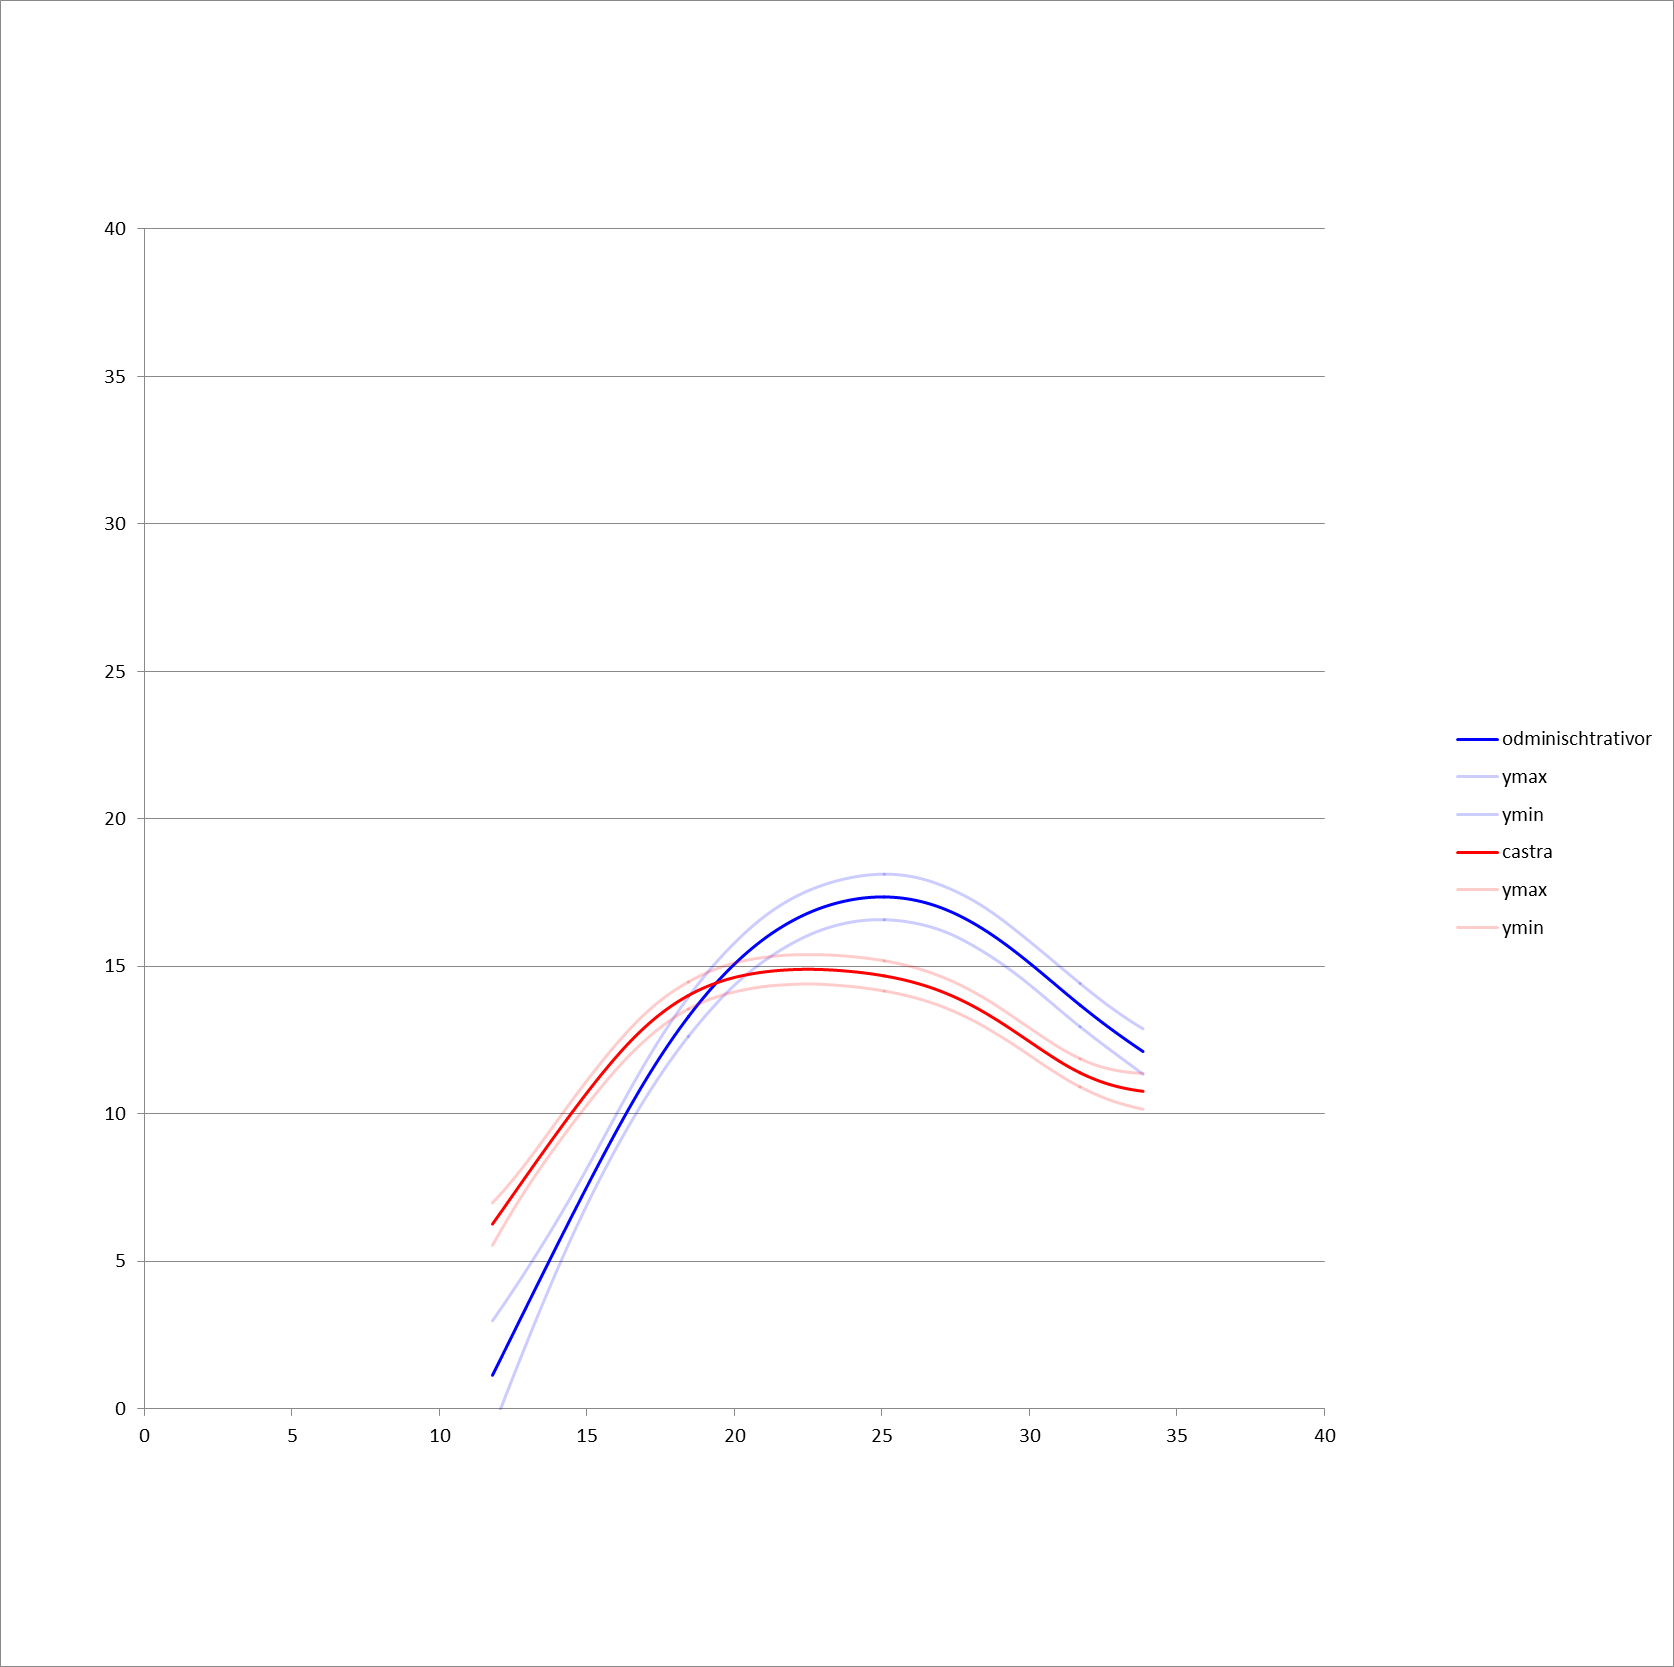
\includegraphics[width=0.4\textwidth]{illustrations/sprea_fig5b}\\
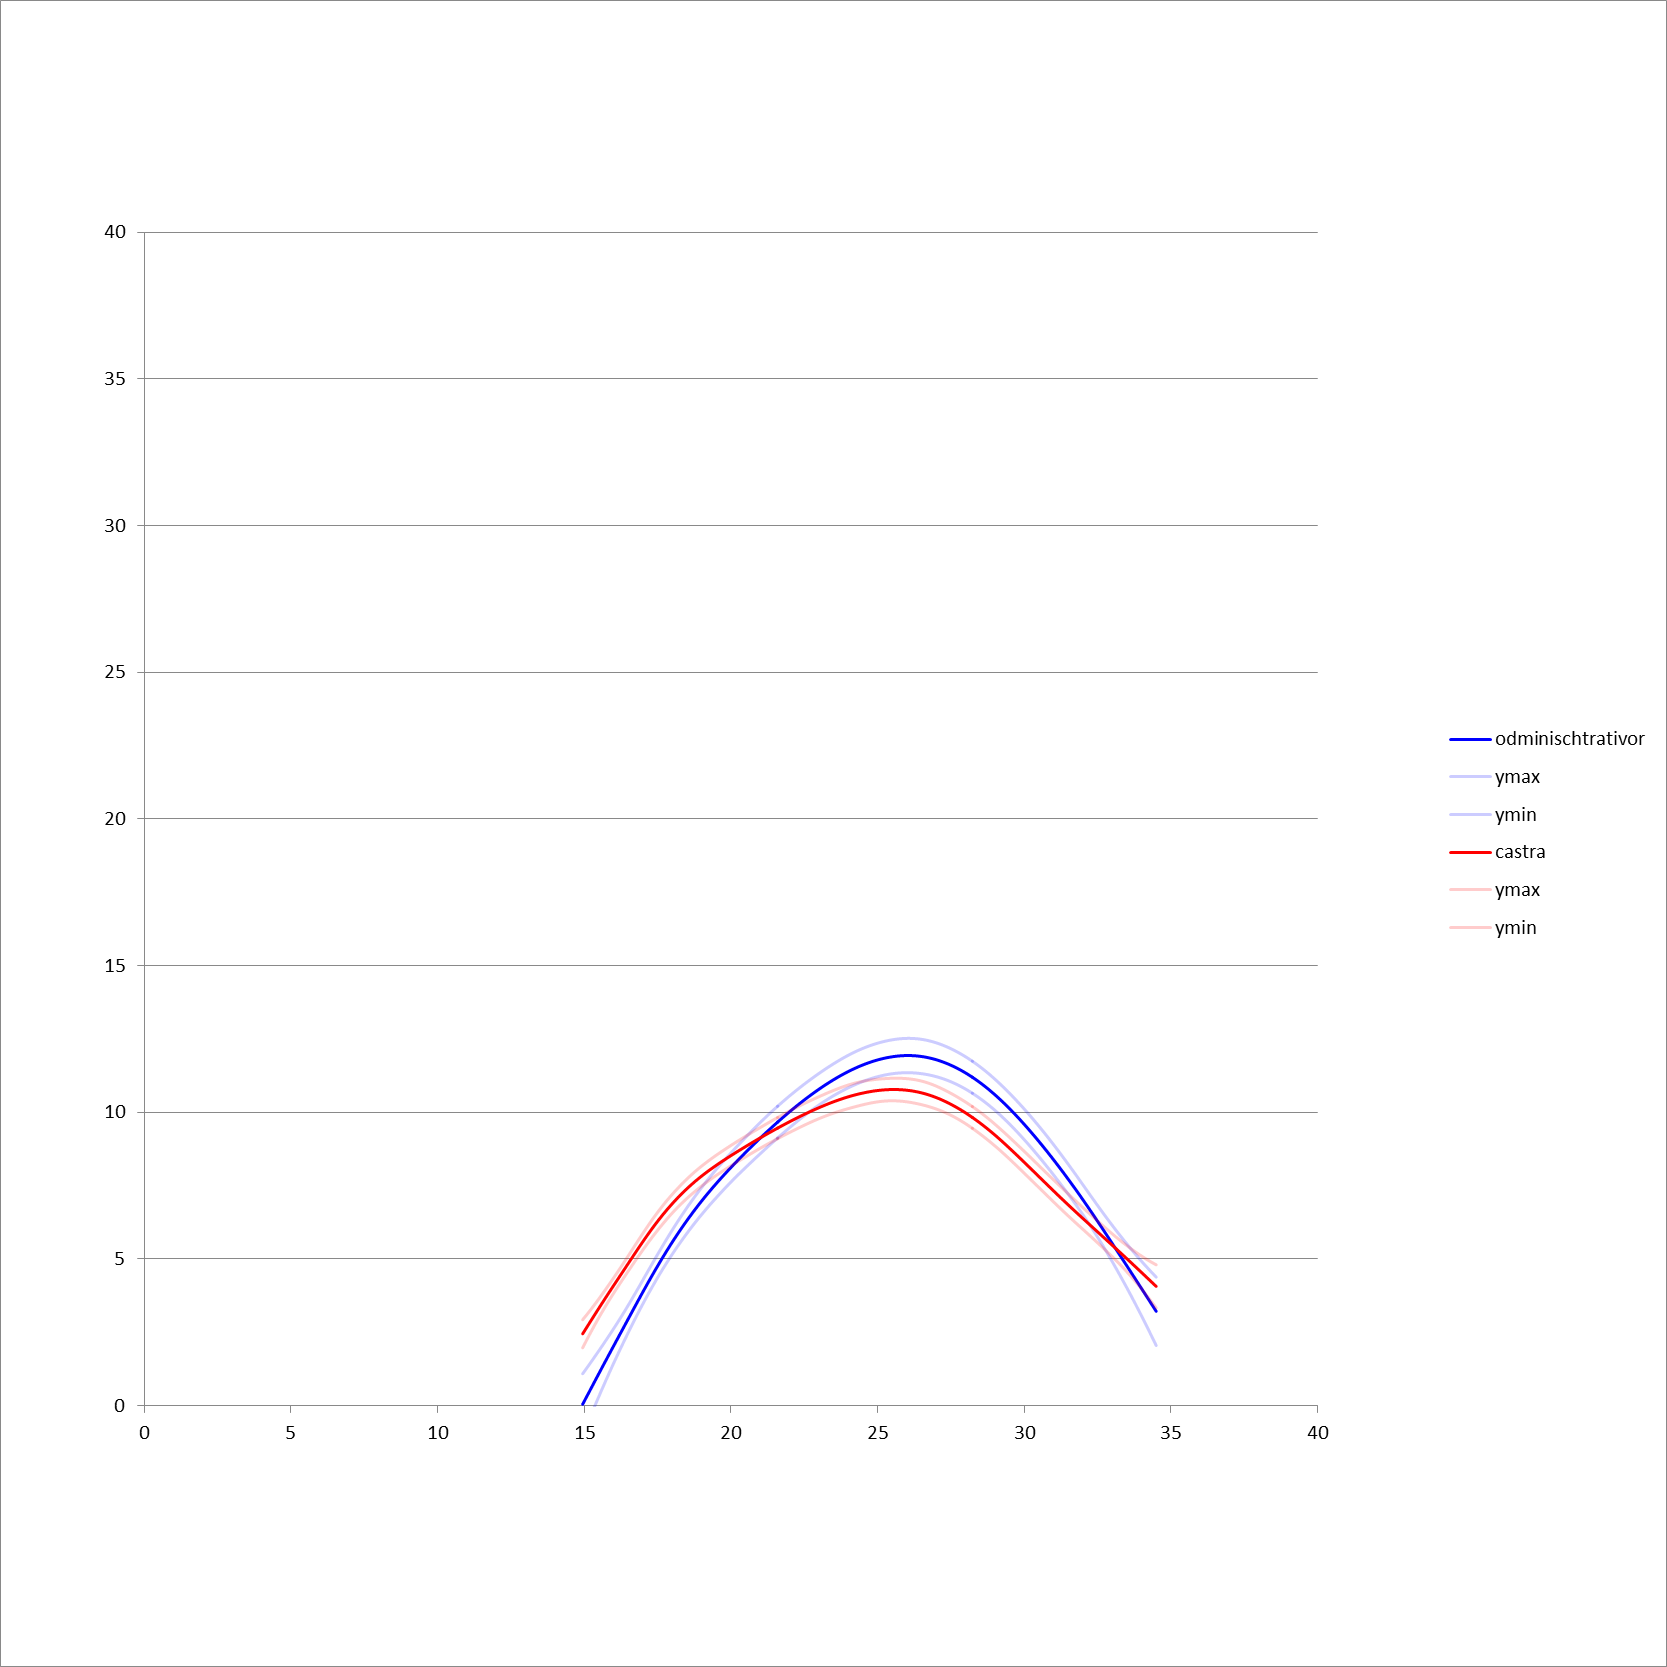
\includegraphics[width=0.4\textwidth]{illustrations/sprea_fig5c}~
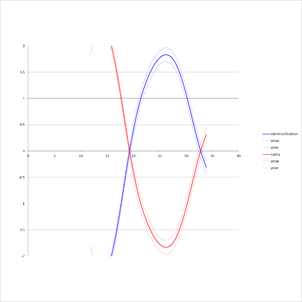
\includegraphics[width=0.4\textwidth]{illustrations/sprea_fig5d}\\
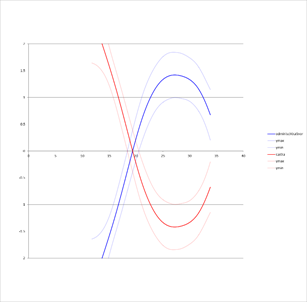
\includegraphics[width=0.4\textwidth]{illustrations/sprea_fig5e}~
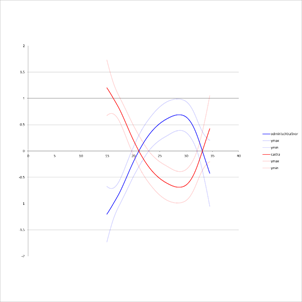
\includegraphics[width=0.4\textwidth]{illustrations/sprea_fig5f}\\
\label{fig:5}   
\caption{Smoothing spline estimate (above) and interaction effects (below) for comparison of the mean curves for /s/ in “castra” (red) and “odminischtrativor” (blue) for subject LS1, LS2, SB2 (from left to right). Tracings for “odminischtrativor” in SB1 were corrupted hence discarded.}
\end{figure}

Elicited data show that concerning the Tyrolean-dominant speaker, smoothing splines for the Italian and the Tyrolean fricative are significantly different and, in particular, that in Italian, the possible retraction is very limited if compared to the shape and position of the tongue for the comparable Tyrolean context. Analogous variation is found in the almost monolingual speaker of Italian who, when pretending to speak Tyrolean, excludes tongue flexion and keeps the body much higher than when speaking Italian. In line with that displayed in \figref{fig:4}, the simultaneous bilingual speaker SB1 appears not to change the overall shape of the tongue but, nevertheless, to articulate significantly different profiles.

According to two independent evaluators, within-speaker articulatory differences displayed in \figref{fig:5} are perceptually relevant and can be reported to Italian [s] and %Tyrolean [ʃ]
respectively. On the contrary, within-speaker articulatory differences shown in Figures 2-4 are statistically significant but perceptually negligible, possibly because of the coincidence of the normalized rear-most points of contact of the tongue. Non-audible s-retraction in Italian as spoken by LS2, SB1 and SB2 – namely the informants in the database who had Tyrolean in their linguistic repertoire – would indicate that irrespective of the rate or age of first exposure to Italian, these speakers do not transfer but %instead control the allophonic alternation /s, ʃ/
characteristic of \textsc{tyr}. Non-perceptible, but UTI-visible gradient articulatory effects nevertheless indicate that, depending on the familiarity with Italian, the production of /s/ in that language by the simultaneous bilingual speakers is less influenced by 
%the /s, ʃ/ 
allophony characteristic of the Tyrolean language.

\section{Conclusion}
At this stage of investigation, the possible indexical value of s-retraction in Italian as spoken by sequential and simultaneous bilinguals from South Tyrol cannot receive a full, positive answer if approached from a ultrasound-tongue-imaging-based socioarticulatory approach, if only because more (varied and accurate) data are needed. Nevertheless, this approach points to promising directions of investigation because there appears to be non-audible differences in tongue positioning between Italian-dominant vs. sequential and simultaneous Italian-Tyrolean bilingual speakers. Seemingly, these differences generate little or no acoustic consequence but might be sociophonetically relevant and need to be scrutinized.

\section*{Acknowledgement}
I thank the editors and two anonymous reviewers for their comments, which helped me to improve the manuscript.

\printbibliography[heading=subbibliography,notkeyword=this]
<<<<<<< HEAD
\end{document}
=======
\end{document}
>>>>>>> 1528c49b69aa568ef669e68c8345d7b1a0c80f19